%! Author = gramic
%! Date = 10.05.24

% Preamble
\begin{flushleft}
    \subsubsection{Maintenance-Tool - AUTOVACUUM}
    \paragraph{Ziel und Zweck}
    Folgende beiden \Gls{AUTOVACUUM}-Parameter sind entscheidend für die Definition, wann \Gls{AUTOVACUUM} startet:
    \begin{description}
        \item \textbf{autovacuum\_vacuum\_threshold}\hfill \\Mindestanzahl geänderter oder gelöschter Tupels die es in einer Tabelle braucht,\\damit \Gls{AUTOVACUUM} startet.\\Der Default liegt bei 50 toten Tuples.
        \item \textbf{autovacuum\_vacuum\_scale\_factor}\hfill \\Definiert, wie Prozent der Datensätze einer Datenbank geändert oder gelöscht werden müssen, bevor vakuumiert wird.
    \end{description}

    Die Grundformel, wann vakuumiert wird, sieht folgendermassen aus:\\
    \(\mathlarger{n\_dead\_tup > (pg\_class.reltuples \times autovacuum\_vacuum\_scale\_factor) + autovacuum\_vacuum\_threshold}\)
\end{flushleft}
\begin{flushleft}
    Der autovacuum\_vacuum\_scale\_factor über den gesamten \Gls{PostgreSQL Cluster} muss nun also mit der Zeit nachjustiert werden.\\
    Dazu wurde obige Formel entsprechend umgestellt, da autovacuum\_vacuum\_threshold grundsätzlich statisch bleibt:
\end{flushleft}
\begin{flushleft}
    \(\mathlarger{\mathlarger{autovacuum\_vacuum\_scale\_factor = \dfrac{(n\_dead\_tup_{max} - autovacuum\_vacuum\_threshold)}{pg\_class.reltuples}}}\)
\end{flushleft}
\begin{flushleft}
    Die Aufgabe von diesem Maintenance-Skripts ist es also nun, einmal pro Tag den autovacuum\_vacuum\_scale\_factor neu zu berechnen.\\
    Da keine Mails versendet werden können, soll bei einem sich geänderten Parameter die generierte HTML-Tabelle auf das Verzeichnis des \Gls{Kubernetes} Nodes gespeichert werden.\\
    Im produktiven Betrieb soll die Tabelle als HTML in die Mail eingefügt werden.
    \paragraph{Funktionsweise}
    In einem ersten Schritt werden alle benötigten Parameter aus der \Gls{PostgreSQL}-Konfiguration oder den entsprechenden Katalogtabellen ausgelesen.\\
    Dies lässt sich mit einem SQL bewerkstelligen, welches wie folgt aufgebaut ist:
    \lstset{style=gra_codestyle}
    \begin{lstlisting}[language=sql, caption=Maintenance-Tool - Parameter - Maintenance-Tool - AUTOVACUUM,captionpos=b,label={lst:maintenannce-tool-parameter-maintenance-tool-autovacuum},breaklines=true]
select
    (
        select
            setting as autovacuum_vacuum_scale_factor
        from pg_settings
        where
            name = 'autovacuum_vacuum_scale_factor'
    ) as autovacuum_vacuum_scale_factor,
    (
        select
            setting as autovacuum_vacuum_threshold
        from pg_settings
        where
            name = 'autovacuum_vacuum_threshold'
    ) as autovacuum_vacuum_threshold,
    (
        select
            sum(reltuples) as reltuples
        from pg_class
    ) as reltuples,
    (
        select
            sender_host
        from pg_stat_wal_receiver
    ) as sender_host
    \end{lstlisting}
\end{flushleft}
\begin{flushleft}
    Anschliessend wird ein Python Dictionary erstellt, welches wiederum in ein pandas DataFrame umgewandelt wird.\\
    Mit der Methode \texttt{to\_html()} wird die Tabelle dann simpel auf das gemountete Host Filesystem geschrieben.\\
    Die Tabelle sieht wie folgt aus:
    \begin{figure}[H]
        \centering
        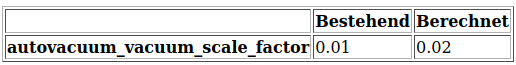
\includegraphics[width=1\linewidth]{source/implementation/construction_implementation/maintenance_tool_autovacuum/autovacuum_result_html_table}
        \caption{\Gls{AUTOVACUUM} - Berechneter autovacuum\_vacuum\_scale\_factor}
        \label{fig:autovacuum_result_html_table}
    \end{figure}
\end{flushleft}
\begin{flushleft}
    Die vollständige Dokumentation ist im \hyperref[subsec:maintenance_autovacuum]{Anhang - Maintenance-Tool - Maintenance-Tool - \Gls{AUTOVACUUM}} zu finden.
\end{flushleft}